%%%%%%%%%%%%%%%%%%%%%%%%%%%%%%%%%%%%%%%%%%%%%%%%%%%%%%%%
%                       Assignment 2                   %
%                                                      %
% Author: Michael P. J. Camilleri					   %
%                                                      %
% Based on the Cleese Assignment Template for Students %
% from http://www.LaTeXTemplates.com.				   %
%                                                      %
% Original Author: Vel (vel@LaTeXTemplates.com)		   %
%													   %
% License:											   %
% CC BY-NC-SA 3.0 									   %
% (http://creativecommons.org/licenses/by-nc-sa/3.0/)  %
% 													   %
%%%%%%%%%%%%%%%%%%%%%%%%%%%%%%%%%%%%%%%%%%%%%%%%%%%%%%%%

%--------------------------------------------------------
%   IMPORTANT: Do not touch anything in this part
\documentclass[12pt]{article}
%%%%%%%%%%%%%%%%%%%%%%%%%%%%%%%%%%%%%%%%%
% Cleese Assignment
% Structure Specification File
% Version 1.0 (27/5/2018)
%
% This template originates from:
% http://www.LaTeXTemplates.com
%
% Author:
% Vel (vel@LaTeXTemplates.com)
%
% License:
% CC BY-NC-SA 3.0 (http://creativecommons.org/licenses/by-nc-sa/3.0/)
% 
%%%%%%%%%%%%%%%%%%%%%%%%%%%%%%%%%%%%%%%%%

%----------------------------------------------------------------------------------------
%	PACKAGES AND OTHER DOCUMENT CONFIGURATIONS
%----------------------------------------------------------------------------------------

\usepackage{lastpage} % Required to determine the last page number for the footer
\usepackage{graphicx} % Required to insert images
\setlength\parindent{0pt} % Removes all indentation from paragraphs
\usepackage[most]{tcolorbox} % Required for boxes that split across pages
\usepackage{booktabs} % Required for better horizontal rules in tables
\usepackage{listings} % Required for insertion of code
\usepackage{etoolbox} % Required for if statements
\usepackage{geometry} % Required for adjusting page dimensions and margins
\usepackage[utf8]{inputenc} % Required for inputting international characters
\usepackage[T1]{fontenc} % Output font encoding for international characters
\usepackage{fancyhdr} % Required for customising headers and footers
\usepackage{xspace}
\usepackage{booktabs}
\usepackage[colorlinks]{hyperref}
\usepackage{etoolbox}

\newcommand{\ie}{i.e.\@\xspace}
\newcommand{\eg}{e.g.\@\xspace}
\newcommand{\notemark}[1]{\textcolor{blue}{N.B.\ \emph{#1}}}
\newcommand{\noteself}[1]{\textcolor{red}{Thought: \emph{#1}}}
\newcommand{\note}[1]{\emph{\textbf{N.B.}\@\xspace#1}}
\newcommand{\hint}[1]{\emph{Hint: #1}}
\newcommand{\half}{$\frac{1}{2}$ }

\newbool{clearnext}		%Running Counter to see if clearing the page or not in the next subquestion.
\newbool{clearon}		%Parameter for specifying whether we will be clearing or not.
\newbool{authoron}		%Parameter to specify whether to show author or not

%----------------------------------------------------------------------------------------
%	Standard Template
%----------------------------------------------------------------------------------------
\geometry{
	paper=a4paper, % Change to letterpaper for US letter
	top=3cm, % Top margin
	bottom=3cm, % Bottom margin
	left=2.5cm, % Left margin
	right=2.5cm, % Right margin
	headheight=14pt, % Header height
	footskip=1.4cm, % Space from the bottom margin to the baseline of the footer
	headsep=1.2cm, % Space from the top margin to the baseline of the header
	%showframe, % Uncomment to show how the type block is set on the page
}
\pagestyle{fancy} % Enable custom headers and footers

%----------------------------------------------------------------------------------------
%	My Changes
%----------------------------------------------------------------------------------------
\lhead{\small\assignmentClass}
\chead{}
\ifbool{authoron}{\rhead{\small{\assignmentAuthorName}}}{\rhead{}}

\lfoot{} % Left footer
\cfoot{} % Centre footer
\rfoot{\small Page\ \thepage\ of\ \pageref{LastPage}} % Right footer

\renewcommand\headrulewidth{0.5pt} % Thickness of the header rule

%----------------------------------------------------------------------------------------
%	MODIFY SECTION STYLES
%----------------------------------------------------------------------------------------

\usepackage{titlesec} % Required for modifying sections

%------------------------------------------------
% Section

\titleformat
{\section} % Section type being modified
[block] % Shape type, can be: hang, block, display, runin, leftmargin, rightmargin, drop, wrap, frame
{\Large\bfseries} % Format of the whole section
{\assignmentQuestionName~\thesection} % Format of the section label
{6pt} % Space between the title and label
{} % Code before the label

\titlespacing{\section}{0pt}{0.5\baselineskip}{0.5\baselineskip} % Spacing around section titles, the order is: left, before and after

%------------------------------------------------
% Subsection

\titleformat
{\subsection} % Section type being modified
[block] % Shape type, can be: hang, block, display, runin, leftmargin, rightmargin, drop, wrap, frame
{} % Format of the whole section
{[\arabic{section}.\arabic{subsection}]} % Format of the section label (\alph{subsection})
{4pt} % Space between the title and label
{} % Code before the label

\titlespacing{\subsection}{0pt}{0.5\baselineskip}{0.5\baselineskip} % Spacing around section titles, the order is: left, before and after

\renewcommand\thesubsection{(\alph{subsection})}

%----------------------------------------------------------------------------------------
%	CUSTOM QUESTION COMMANDS/ENVIRONMENTS
%----------------------------------------------------------------------------------------

% Environment to be used for each question in the assignment
\newenvironment{question}[1]{
	\ifbool{clearon}{\clearpage}{}
	\global\setbool{clearnext}{false}
	\vspace{0.5\baselineskip} % Whitespace before the question
	\section{: #1}
	\lfoot{\small\itshape\assignmentQuestionName~\thesection~continued on next page\ldots} % Set the left footer to state the question continues on the next page, this is reset to nothing if it doesn't (below)
}{
	\lfoot{} % Reset the left footer to nothing if the current question does not continue on the next page
}

%------------------------------------------------

% Environment for inter-subquestion texts (no arguments)
\newenvironment{interquestiontext}{
	\ifbool{clearon}{\ifbool{clearnext}{\clearpage}{}}{}
	\global\setbool{clearnext}{false}
}{
}

%------------------------------------------------


%------------------------------------------------

% Environment for subquestions, takes 1 argument - the name of the section
\newenvironment{subquestion}[1]{
	\ifbool{clearon}{\ifbool{clearnext}{\clearpage}{}}{}
	\global\setbool{clearnext}{true}
	\subsection{#1}
}{
}

%------------------------------------------------

% Command to print a question sentence
\newcommand{\questiontext}[1]{
	\textbf{#1}
	\vspace{0.5\baselineskip} % Whitespace afterwards
	\global\setbool{clearnext}{false}
}

%------------------------------------------------
% Command to print a  Marking Scheme box.
\newcommand{\marking}[1]{
	\begin{tcolorbox}[colback=green!5!white,enhanced]
		\textbf{Marking Scheme:}#1
	\end{tcolorbox}
}

%------------------------------------------------

% Command to print a box that breaks across pages with the space for a student to answer
\newcommand{\model}[1]{
	\begin{tcolorbox}[enhanced]
		\textbf{Model Answer}:#1
	\end{tcolorbox}
}

\newcommand{\answerbox}[2]{
	\begin{tcolorbox}[enhanced, height=#1]
		#2
	\end{tcolorbox}
}

%------------------------------------------------

% Command to print an assignment section title to split an assignment into major parts
\newcommand{\assignmentSection}[1]{
	{
		\centering % Centre the section title
		\vspace{2\baselineskip} % Whitespace before the entire section title
		
		\rule{0.8\textwidth}{0.5pt} % Horizontal rule
		
		\vspace{0.75\baselineskip} % Whitespace before the section title
		{\LARGE \MakeUppercase{#1}} % Section title, forced to be uppercase
		
		\rule{0.8\textwidth}{0.5pt} % Horizontal rule
		
		\vspace{\baselineskip} % Whitespace after the entire section title
	}
}

%----------------------------------------------------------------------------------------
%	TITLE PAGE
%----------------------------------------------------------------------------------------

\title{
	\thispagestyle{empty} 		% Suppress headers and footers
	\vspace{0.01\textheight} 	% Whitespace before the title
	\textbf{\assignmentClass:\\ \assignmentTitle}\\[4pt]
	\ifbool{authoron}{\assignmentAuthorName}{
	\ifdef{\assignmentDueDate}{{\small Due\ on\ \assignmentDueDate}\\}{}
	{\large \textit{\assignmentWarning}}
	\vspace{0.01\textheight}} % Whitespace before the author name
}

\ifbool{authoron}{\author{Student: \textbf{\assignmentAuthorName}}}{}
\date{} % Don't use the default title page date field





% Options for Formatting Output

\global\setbool{clearon}{true} %
\global\setbool{authoron}{true} %



\newcommand{\assignmentQuestionName}{Question}
\newcommand{\assignmentTitle}{Assignment\ \#2}

\newcommand{\assignmentClass}{IAML -- INFR10069 (LEVEL 10)}

\newcommand{\assignmentWarning}{NO LATE SUBMISSIONS} % 
\newcommand{\assignmentDueDate}{Friday,\ November\ 15,\ 2019 @ 16:00}
%--------------------------------------------------------

%--------------------------------------------------------
%   IMPORTANT: Specify your Student ID below [You will need to uncomment the line, else compilation will fail]. Make sure to specify your student ID correctly, otherwise we may not be able to identify your work and you will be marked as missing.
\newcommand{\assignmentAuthorName}{s1712653}
%--------------------------------------------------------

\begin{document}
\maketitle
\thispagestyle{empty}



%%%%%%%%%%%%%%%%%%%%%%%%%%%%%%%%%%%%%%%%%%%%%%%%%%%%%%%%%%%%%%%%%%%%%%%%%%%%%%
%============================================================================%
%%%%%%%%%%%%%%%%%%%%%%%%%%%%%%%%%%%%%%%%%%%%%%%%%%%%%%%%%%%%%%%%%%%%%%%%%%%%%%


\assignmentSection{Part A: 20-NewsGroups [60 Points]}




\begin{question}{(10 points) Exploratory Analysis}

\questiontext{We will begin by exploring the Dataset to get some insight about it.}



\begin{subquestion}{(5 points) Focusing first on the training set, summarise the key features/observations in the data: focus on the dimensionality, data ranges, feature and class distribution and report anything out of the ordinary. What are the typical values of the features like?}


\answerbox{12em}{
    The training set consists of 5648 observations, each with a dimensionality of 1000. Each attribute of an observation corresponds to a word, and its value is the TF-IDF weight of that word, which ranges from 0 to 1 in this particular data set. The average values of each attribute range from 0.0001 to 0.0252. The most common attribute value is 0 as not all words appear in a document at once. There is an uneven class distribution as class 7 is almost half as frequent as all of the other classes, this will impact our model classification accuracy as words that belong to class 7 might be misclassified. The distribution of the mean value of each attribute resembles a positively skewed normal distribution with mean roughly around 0.0025.
}



\end{subquestion}


\begin{subquestion}{(3 points) Looking now at the Testing set, how does it compare with the Training Set (in terms of sizes and feature-distributions) and what could be the repurcussions of this?}


\answerbox{10em}{
    The testing set consists of 1883 observations with a similar attribute value range to the training set. The class distribution also closely resembles the training set where class 1 to 6 have similar frequencies while class 7 is almost half as frequent as the other classes. The distribution of the mean value of each attribute also resembles the distribution observed on the training set, this supports the assumption for machine learning where the training and testing sets should be sampled from the same distribution, thus lowering the amount of bias from the testing set.
}



\end{subquestion}

\begin{subquestion}{(2 points) Why do you think it is useful to consider TF-IDF weights as opposed to just the frequency of times a word appears in a document as a feature?}



\answerbox{10em}{
    The desired model should take into account how relevant each word is to each document, that is, the words which would most help a human better understand a document without reading it all. Relevant words do not necessarily mean the most frequent words, for example, stopwords which are frequent while not offering much meaning. Thus it is important to not only consider the document but the dataset as a whole, as we want to distinguish words that are meaningful to a particular document and not words that appear the most, which TF-IDF tries to measure.
}



\end{subquestion}



\end{question}


%============================================================================%

\begin{question}{\label{Q_UNSUP_LEARN}(24 points) Unsupervised Learning}

\questiontext{We will now explore the documents in some detail by way of clustering.}



\begin{subquestion}{(2 points) The K-Means algorithm is non-deterministic. Explain why this is, and how the final model is selected in the SKLearn implementation of \href{https://scikit-learn.org/stable/modules/clustering.html}{KMeans}.}



\answerbox{8em}{
    The non-deterministic nature of the K-Means algorithm comes from its random selection of starting centroids, this means that depending on the choice of the starting centroids the algorithm could give rise to entirely different models of the data. The SKLearn implementation of K-Means selects the final model based on which one minimizes Inertia the most.
}



\end{subquestion}


\begin{subquestion}{(1 point) One of the parameters we need to specify when using k-means is the number of clusters. What is a reasonable number for this problem and why?}



\answerbox{5em}{
    The observations in the data set each belong to 1 of 8 different classes. This could imply that the observations from each class have similar values in the feature space, thus a reasonable number for this data set could be the number of classes: 8.
}



\end{subquestion}


\begin{subquestion}{(5 points) We will use the Adjusted Mutual Information (AMI) \ie \href{https://scikit-learn.org/stable/modules/clustering.html\#mutual-info-score}{\texttt{adjusted\_mutual\\\_info\_score}} between the clusters and the true (known) labels to quantify the performance of the clustering. Give an expression for the MI in terms of entropy. In short, describe what the MI measures about two variables, why this is applicable here and why it might be difficult to use in practice. \hint{MI is sometimes referred to as Information Gain: note that you are asked only about the standard way we defined MI and not the AMI which is adjusted for the size of the domain and for chance agreement.}}



\answerbox{16em}{
    Mutual information, $\mathrm{MI}$, of known variables $U$ and $V$ can be calculated as $\mathrm{MI}(U,V)=\mathrm{H}(U)-\mathrm{H}(U|V)$, where $\mathrm{H}(X)$ is the entropy of variable $X$. Mutual information measures how much one variable tells us about the other, thus it is the reduction in uncertainty about variable $X$ after having observed variable $Y$. Mutual Information is applicable to this problem as we are trying to measure how much information is shared, and therefore the accuracy, between predicted labels and the ground truth of the data regardless of the ordering of the clusters produced by the algorithm. In practice it is difficult to use as it requires for the true labels of the data to be known, which might not be available in practice or requires them to be manually assigned.
}



\end{subquestion}

\begin{subquestion}{(4 points) Fit K-Means objects with \texttt{n\_clusters} ranging from 2 to 12. Set the random seed to 1000 and the number of initialisations to 50, but leave all other values at default. For each fit compute the adjusted mutual information (there is an SKLearn \href{https://scikit-learn.org/stable/modules/generated/sklearn.metrics.adjusted_mutual_info_score.html}{function} for that). Set \texttt{average\_method=`max'}. Plot the AMI scores against the number of clusters (as a line plot).}



\answerbox{40em}{
    \begin{center}
        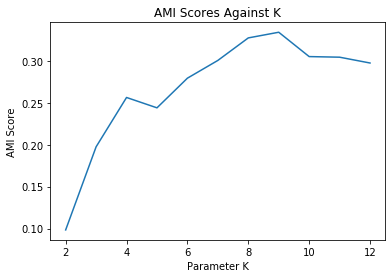
\includegraphics[width=0.9\textwidth]{figure1.png}
    \end{center}
}



\end{subquestion}

\begin{subquestion}{(3 points) Discuss any trends and interesting aspects which emerge from the plot. Does this follow from your expectations?}



\answerbox{10em}{
    The $\mathrm{AMI}$ seems to grow larger as $K$ increases up to a point. Contrary to what is expected the highest $\mathrm{AMI}$ is not observed when $K=8$ (the number of classes), but instead from $K=9$, which could indicate that the data set is best modeled by 9 different classes. The $\mathrm{AMI}$ starts trending down for $K>9$. There also seems to be an unexpected decrease in $\mathrm{AMI}$ from $K=4$ to $K=5$.
}



\end{subquestion}

\begin{subquestion}{\label{Q_CLUSTER_FOUR}(6 points) Let us investigate the case with four (4) clusters in some more detail. Using seaborn's \href{https://seaborn.pydata.org/generated/seaborn.countplot.html}{\texttt{countplot}} function, plot a bar-chart of the number of data-points with a particular class (encoded by colour) assigned to each cluster centre (encoded by position on the plot's x-axis). As part of the cluster labels, include the total number of data-points assigned to that cluster.}



\answerbox{40em}{
    \begin{center}
        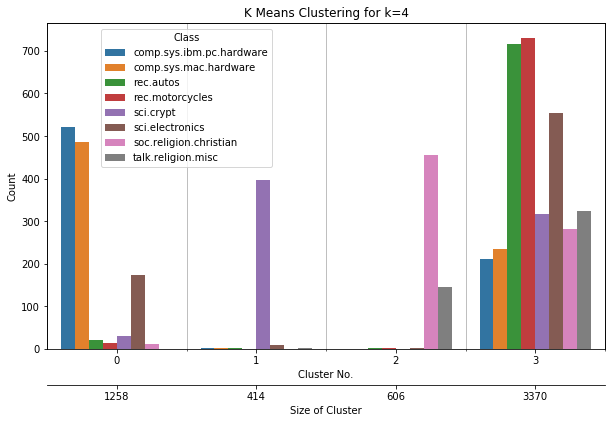
\includegraphics[width=1\textwidth]{figure2.png}
    \end{center}
}



\end{subquestion}

\begin{subquestion}{(3 points) How does the clustering in Question\ref{Q_UNSUP_LEARN}:\ref{Q_CLUSTER_FOUR} align with the true class labels? Does it conform to your observations in Q 2(e)?}



\answerbox{14em}{
    The clustering for $K=4$ is not very accurate as all observations belonging to a particular true class label are not all in 1 cluster. Most observations belonging to a class seem to be mostly spread out over two different clusters with the exception of $rec.motorcycles$ and $rec.autos$ which are mostly assigned to a single cluster. The cluster sizes are also very uneven with the smallest clusters only containing 1 or 2 classes on the majority, while the largest cluster has almost 6 times the samples as the smallest cluster and also contains significant amounts of samples from all classes. The result is mostly expected as the $\mathrm{AMI}$ score for $K=4$ indicates that the data is not well modelled by 4 clusters as observed in the previous questions.
}



\end{subquestion}



\end{question}

%============================================================================%

\begin{question}{(26 points) Logistic Regression Classification}
\label{Q_LR_NG}
\questiontext{We will now try out supervised classification on this data. We will focus on Logistic Regression and measure performance in terms of the \href{https://scikit-learn.org/stable/modules/generated/sklearn.metrics.f1_score.html}{F1} score (familiarise yourself with this score which is related to the precision and recall scores that we learnt about in class).}



\begin{subquestion}{(3 points) What is the F1-score, and why is it preferable to accuracy in our problem? How does the macro-average work to extend the score to multi-class classification?}



\answerbox{8em}{
    The $\mathrm{F1}$ Score is the weighted average of the precision and recall of a model. It takes into account both false positives and false negatives, as well as taking into account class imbalance, which is the case for this data set, thus it is prefered over accuracy. The macro-average extends the score to handle multiple classes by calculating the metrics for each label and then finding their unweighted mean as per the SKlearn documentation for the function $\mathrm{f1\_score}$.
}



\end{subquestion}


\begin{subquestion}{(2 points) As always we start with a simple baseline classifier. Define such a classifier (indicating why you chose it) and report its performance on the \textbf{Test} set. Use the `macro' average for the \texttt{f1\_score}.} %\hint{For the baseline, the classifier should use only the target labels.}



\answerbox{8em}{
    The baseline classifier used will be one that classifies all test samples as the class that occured most often in the training set, $i.e$ the class with the highest prior probability. This is a useful baseline as it allows us to compare it to more complex models. The $\mathrm{F1}$ Score of this model on the test set is: $0.029$.
}



\end{subquestion}

\begin{subquestion}{(3 points) We will now train a \href{https://scikit-learn.org/stable/modules/generated/sklearn.linear_model.LogisticRegression.html}{LogisticRegression} Classifier from SKLearn. By referring to the documentation, explain how the Logistic Regression model can be applied to classify multi-class labels as in our case. \hint{Limit your explanation to methods we discussed in the lectures.}}



\answerbox{9em}{
    To extend Logistic Regression for multi-class problems, first a weight vector $w_k$ is created for each class, then the $\mathrm{softmax}$ function is used to calculate the probability that a feature vector belongs to a class, $P(y=k|x)$, thus assigning each feature vector to a class. The model is then optimized to minimize the log loss, in this case the $\mathrm{L}$-$\mathrm{BFGS}$ algorithm will be used as the optimization method.
}



\end{subquestion}

\begin{subquestion}{(4 points) Train a Logistic Regressor on the training data. Set \texttt{solver=`lbfgs'}, \texttt{multi\_class=`multinomial'} and \texttt{random\_state=0}. Use the Cross-Validation object you created and report the average validation-set F1-score as well as the standard deviation. Comment on the result.}



\answerbox{9em}{
    The average of the $\mathrm{F1}$ Scores calculated from the 10 folds of the training set is: $0.669$, while the standard deviation of the $\mathrm{F1}$ Scores is: $0.017$. The logistic regression model trained on each fold has a significantly higher average $\mathrm{F1}$ Score than the baseline classifier, while having a decently high average $\mathrm{F1}$ Score itself. The $\mathrm{F1}$ Scores calculated also have a low standard deviation indicating that the trained model is precise.
}



\end{subquestion}

\begin{subquestion}{\label{Q_LOG_REG_PLT}(5 points) We will now optimise the Regularisation parameter $C$ using cross-validation. Train a logistic regressor for different values of $C$: in each case, evaluate the F1 score on the training and validation portion of the fold. That is, for each value of $C$ you must provide the training set and validation-set scores per fold and then compute (and store) the average of both over all folds. Finally plot the (average) training and validation-set scores as a function of $C$. \hint{Use a logarithmic scale for $C$, spanning 19 samples between $10^{-4}$ to $10^5$.}}



\answerbox{40em}{
    \begin{center}
        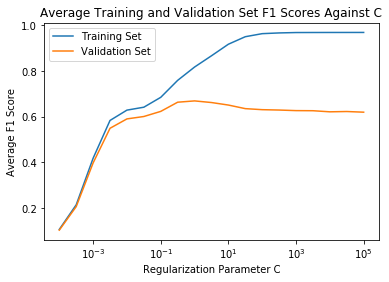
\includegraphics[width=1\textwidth]{figure3.png}
    \end{center}
}



\end{subquestion}

\begin{subquestion}{(7 points) What is the optimal value of $C$ (and the corresponding score)? How did you choose this value? By making reference to the effect of the regularisation parameter $C$ on the optimisation, explain what is happening in your plot from Question \ref{Q_LR_NG}:\ref{Q_LOG_REG_PLT} \hint{Refer to the documentation for $C$ in the \href{https://scikit-learn.org/stable/modules/generated/sklearn.linear_model.LogisticRegression.html}{LogisticRegression} page on SKLearn}.}



\answerbox{11em}{
    The optimal value of $C$ is $1$. This value was chosen as it gives rise to the highest average $\mathrm{F1}$ Score on the validation set. As per the SKlearn documentation, $C$ is the inverse regularization parameter defined as $C=\frac{1}{\lambda}$, where $\lambda$ is the lambda regulator. The effect of changing the value of $C$ can be seen in the plot above, where regularizing too little causes the convergence parameters to not be acertained and therefore leads to a low average $\mathrm{F1}$ Score for the training and validation set, while regularizing too much leads to overfitting of the training data, leading to a higher average $\mathrm{F1}$ Score for the training set while lowering the $\mathrm{F1}$ Score for new data.
}



\end{subquestion}

\begin{subquestion}{(2 points) Finally, report the score of the best model on the test-set, after retraining on the entire training set (that is drop the folds). \hint{You may need to set \texttt{max\_iter = 200}.} Comment briefly on the result.}



\answerbox{7em}{
    The $\mathrm{F1}$ Score for the best model, logistic regression classifier with regularization parameter $C=1$, on the test set is: $0.675$. This result is significantly larger compared to the baseline classifier, and is a decently large $\mathrm{F1}$ Score itself, which indicates that it is classifying the test set well.
}



\end{subquestion}


\end{question}




%============================================================================%




%%%%%%%%%%%%%%%%%%%%%%%%%%%%%%%%%%%%%%%%%%%%%%%%%%%%%%%%%%%%%%%%%%%%%%%%%%%%%%
%============================================================================%
%%%%%%%%%%%%%%%%%%%%%%%%%%%%%%%%%%%%%%%%%%%%%%%%%%%%%%%%%%%%%%%%%%%%%%%%%%%%%%

\clearpage

\assignmentSection{Part B: Bristol Air-Quality [90 points]}




\begin{question}{\label{Q_EXPLORATORY}(30 Points) Exploratory Analysis}

\questiontext{We will begin by exploring the Dataset to familiarise ourselves with it.}



\begin{subquestion}{(6 points) Summarise the key features/observations in the data: describe the purpose of each column and report (briefly) also on the dimensionality/ranges (ballpark figures only, and how they compare across features) and number of sites, and identify anything out of the ordinary/problematic: \ie look out for missing data and negative values. Why are the latter unreasonable in such a dataset? \hint{Refer to the documentation for how to interpret the pollutant values.}}



\answerbox{13em}{
    The data set contains 1306757 observations, each corresponting to a reading of 3 pollutants $(\mathrm{NO}_x, \mathrm{NO}_2, \mathrm{NO})$, with values ranging from -31.08 to 2164.25 across all pollutants, at one of 18 sites, labeled from 0 to 17, along with the latitude, ranging from 51.43 to 51.49 degrees, and logitude, ranging from -2.69 to -2.54 degrees, of that site and the date, ranging from the year 2007 to 2019, and time, ranging from 0AM to 12PM in 1 hour intervals, the reading was made. The data has a dimension of 7, however it contains observations with missing values, depicted as $\mathrm{NaN}$, as well as negative values for the pollutant readings. Having pollutant reading with negative values in this dataset is unreasonable as there is no real world interpretation of a negative reading of a pollutant and therefore doesn't have any meaning.
}



\end{subquestion}

\begin{subquestion}{(6 points) Repeat the same analysis but this time on a per-site basis. Provide a table with the number of samples and percentage of problematic samples (negative and missing) in each site. To report numbers, count a row which has at least one missing entry
as having missing data, and similarly for negative entries. \hint{Pandas has a handy method, \texttt{to\_latex()}, for generating a latex table from a dataframe.}}



\answerbox{17em}{
    \begin{tabular}{lrrrrrr}
        \toprule
        SiteID &            0 &              1 &             2 &             3 &             4 &              5 \\
        Count              &  6446 &  163111 &  62990 &  25464 &  74787 &  113952 \\
        \% Missing  &     1.613404 &       6.290195 &      4.348309 &     77.332705 &      2.068541 &       8.828279 \\
        \% Negative &     0 &       0 &      0.004763 &      0.777568 &      0.005349 &       0 \\
        \midrule
        SiteID &             6  &             7  &            8  &            9  &            10 &            11 \\
        Count              &  142141 &  115162 &  43824 &  22071 &  96407 &  20693 \\
        \% Missing  &       7.444017 &       4.194960 &     21.056955 &      5.301074 &      3.589988 &      1.904026 \\
        \% Negative &       0.002814 &       0.277869 &      0 &      0 &      0.004149 &      0.086986 \\
        \midrule
        SiteID &            12 &            13 &            14 &      15 &             16 &            17 \\
        Count              &  45240 &  12423 &  113951 &  2712 &  154331 &  91053 \\
        \% Missing  &     17.484527 &     51.461000 &      10.53172 &   100.0 &       6.530768 &      6.271073 \\
        \% Negative &      0 &      0.016099 &       0 &     0 &       0.013607 &      0.002197 \\
    \end{tabular}
}



\end{subquestion}

\begin{subquestion}{(4 points) Briefly summarise how the sites compare in terms of number of samples and amount of problematic samples.}



\answerbox{11em}{
    The number of samples belonging to each of the 18 sites varies greatly with the smallest number of samples in site 15, with 2712 samples, and the largest number of samples in site 1, with 163111 samples. All sites contain problematic samples, making up less than 10\% of the majority of all sites, however sites 3, 8, 13 and 15 contain significantly more problematic samples, with site 15 being made up of only problematic samples. Out of the 2 types of problematic samples, missing samples occur significantly more than negative samples.
}



\end{subquestion}

\begin{subquestion}{(3 points) Given that the columns are all oxides of nitrogen and hence we expect them to be related, we will now look at correlations in our data. This will also be useful in determining how well we can predict any one of the readings from the other two. Remove the data from sites 3 and 15 and compute the \textbf{Pearson} correlation coefficient between each of the three pollutant columns on the remaining data. Visualise the coefficients between each pair of columns in a table.}



\answerbox{10em}{
    \begin{tabular}{lrrr}
        \toprule
        {} &       NOx &       NO2 &        NO \\
        \midrule
        NOx &  1.000000 &  0.878016 &  0.988019 \\
        NO2 &  0.878016 &  1.000000 &  0.807853 \\
        NO  &  0.988019 &  0.807853 &  1.000000 \\
        \bottomrule
    \end{tabular}
        
}



\end{subquestion}

\begin{subquestion}{(2 points) Comment on the level of correlation between each pair of pollutants.}



\answerbox{7em}{
    From the data set, each pollutant seems to have a significant positive correlation with every other pollutant. Out of all the pairs $\mathrm{NO}_x$ and $\mathrm{NO}$ exhibit the strongest positive correlation, while $\mathrm{NO}_x$ and $\mathrm{NO}_2$ exhibit the least strongest positive correlation. This could indicate that all 3 pollutants have a positive correlation with each other.
}



\end{subquestion}



\begin{subquestion}{\label{CORRELATIONS}(5 points) For each of the three pollutants, compute the Pearson correlation between sites. \hint{You will need to remove the `Date Time' column and then group by the first level of the columns.} Then plot these as three heatmaps: show the values within the figures. \hint{Use the method \texttt{plot\_matrix()} from \texttt{mpctools.extensions.mplext}.}}



\answerbox{40em}{
    \begin{center}
        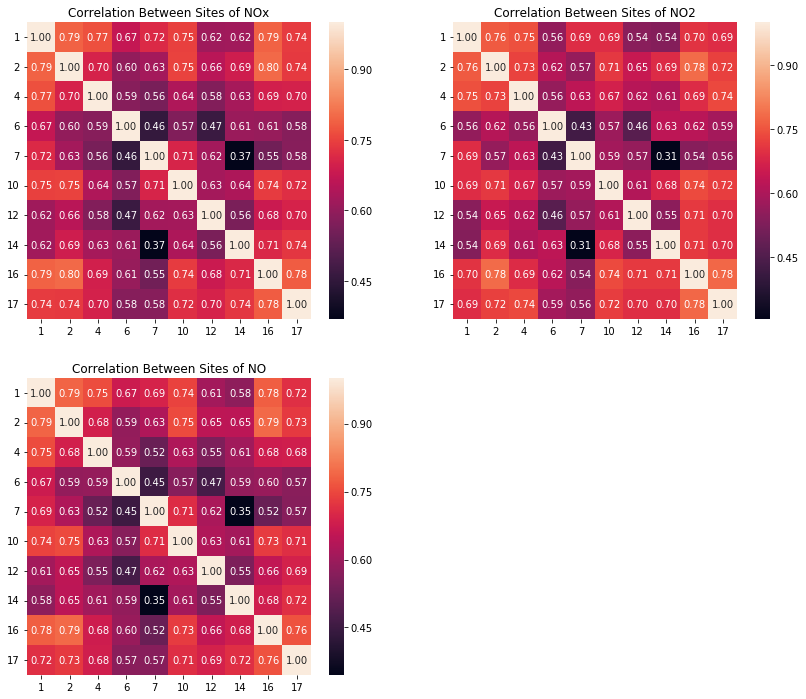
\includegraphics[width=1.04\textwidth]{figure4_2.png}
    \end{center}
}



\end{subquestion}

\begin{subquestion}{(4 points) Comment briefly on your observations from Question \ref{Q_EXPLORATORY}:\ref{CORRELATIONS}: start by summarising the results from the NO gas and then comment on whether the same is observed in the other gases or if there is something different.}



\answerbox{12em}{
    As seen from the heatmap plot for $\mathrm{NO}$ from the last question the pearson correlation coefficient between each pair of sites are all greater than 0, meaning that they all exhibit positive correlation. Some sites, however, show a much weaker positive correlation when paired with all the other sites, particularly sites 6, 7, 12 and 14, with the smallest correlation coefficient arising from the pair 14 and 7. The other 2 heatmaps show similar patterns, however in the heatmap for $\mathrm{NO}_2$, the correlation between sites 10 and 7 is much lower compared to the other two plots.
}



\end{subquestion}

\end{question}


%============================================================================%

\begin{question}{(19 Points) Principal Component Analysis}

\questiontext{One aspect which we have not yet explored is the temporal nature of the data. That is, we need to keep in mind that the readings have a temporal aspect to them which can provide some interesting insight. We will explore this next.}



\begin{subquestion}{(1 point) Plot the first 5 lines of data (plot each row as a single line-plot).}



\answerbox{40em}{
    \begin{center}
        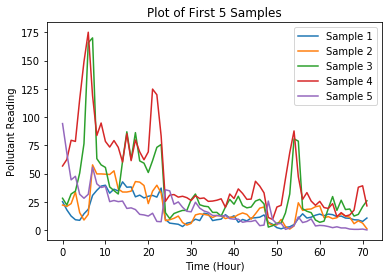
\includegraphics[width=1.0\textwidth]{figure5.png}
    \end{center}
}



\end{subquestion}



\begin{subquestion}{(5 points) We will focus first on data solely from Site 1. Extract the data from this site, and run PCA with the number of components set to 72 for now. Set the \texttt{random\_state=0}. On a single graph plot: (i) the percentage of the variance explained by each principal component (as a bar-chart), (ii) the cumulative variance (line-plot) explained by the first $n$ components: (\hint{you should use \href{https://matplotlib.org/3.1.1/api/_as_gen/matplotlib.axes.Axes.twinx.html}{\texttt{twinx()}} to make the plot fit}), \textsl{and}, (iii) mark the point at which the number of components collectively explain at least 95\% of the variance (using a vertical line). \hint{Number components starting from 1.}}



\answerbox{40em}{
    \begin{center}
        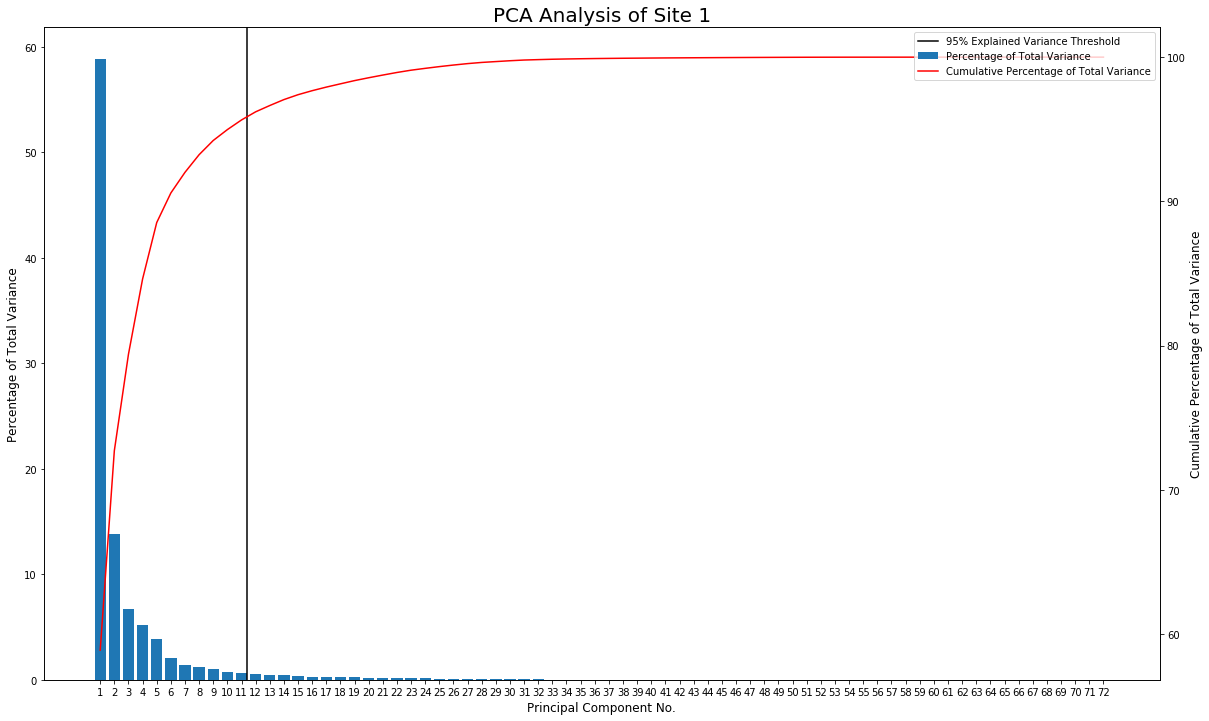
\includegraphics[width=1.039\textwidth]{figure6.png}
    \end{center}
}



\end{subquestion}

\begin{subquestion}{(2 points) Interpret and summarise the above plot.}



\answerbox{9em}{
    As seen from the vertical bars in the plot from the previous question, the first principal component explains more of the total variance than all of the other components combined, thus only 11 principal components are needed to explain 95\% of the total variance. The red line shows the cumulative percentage of the total variance over all 72 principal components, with the cumulative sum being the total variance of the original data.
}



\end{subquestion}


\begin{subquestion}{(5 points) Generate three figures, one for the mean and one for each of the first 2 principal components: in each, plot the mean/component as three lines, one for each pollutant throught one day cycle. \hint{You will need to reshape the components appropriately.}}



\answerbox{50em}{
    \begin{center}
        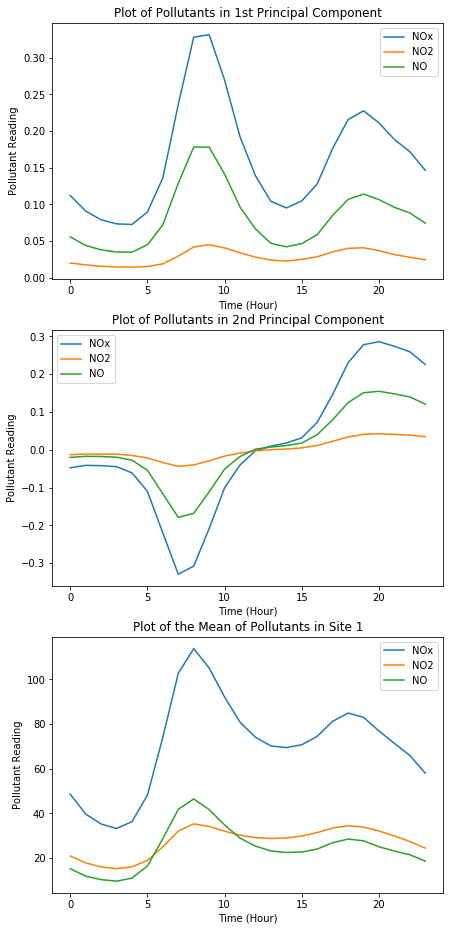
\includegraphics[width=0.66\textwidth]{figure7.png}
    \end{center}
}



\end{subquestion}

\begin{subquestion}{(6 points) Focusing on the mean and first principal component, are there any significant patterns which emerge throughout the day? \hint{Think about car usage throughout the day.} What is different when interpreting the mean versus the first component? \hint{Do peaks signify the same thing in both cases?} Looking at the principal components only, are there any significant differences between the pollutants? Why could this be happening? \hint{You can refer to one of the limitations of PCA.}}



\answerbox{16em}{
    Comparing the plot of the mean and the 1st principal component, a pattern can be seen on the amount of pollutants throughout the day, namely pollutant readings increase significantly around 9AM before decreasing, and then increase significantly again around 7PM, before decreasing again. This could be due to pollution from cars, as there is an increase in use during rush hours. The issue with comparing the mean and the 1st principal component, is that the values in the mean correspond to pollutant readings, whilst in the 1st principal component they corresponds to the direction of greatest variance in the feature space of site 1, thus they don't correspond to the same thing. There are no significant differences between pollutants when comparing the the first 2 principal components, this could be due to the fact that PCA is scale variant and thus is affected by the scale of the data. This can be solved by normalizing the data beforehand, however this was not done.
}



\end{subquestion}

\end{question}

%============================================================================%


\begin{question}{\label{Q_LR_BA}(41 points) Regression}


\questiontext{Given our understanding of the correlation between signals and sites, we will now attempt to predict the NOx level for Site 17 given the value at the other sites. We will evaluate our models using the Root Mean Squared Error (RMSE) \ie the square root of the \href{https://scikit-learn.org/stable/modules/generated/sklearn.metrics.mean_squared_error.html}{mean\_squared\_error} score by sklearn.}



\begin{subquestion}{(2 points) First things first: since we are dealing with a supervised task, we will need to split our data into a training and testing set. Furthermore, since some of our regressors will involve hyper-parameter tuning, we will also need a validation set. Use the \texttt{multi\_way\_split()} method from \texttt{mpctools.extensions.skext} to split the data into a Training (60\%), Validation (15\%) and Testing (25\%) set: use the \href{https://scikit-learn.org/stable/modules/generated/sklearn.model_selection.ShuffleSplit.html}{ShuffleSplit} object from sklearn for the \texttt{splitter}. Set the random state to 0. \hint{The method gives you the indices of the split for each set, which can then be applied to multiple matrices.} Report the sizes of each dataset.}



\answerbox{4em}{
    Size of training set: 8937, size of validation set: 2234, size of testing set: 3724. All sets have a dimension of 9.
}



\end{subquestion}

\begin{subquestion}{(4 points) Let us start with a baseline. By using only the $y$-values, what baseline regressor can you define (indicate what it does)? Implement it and report the RMSE on the training and validation sets. Interpret this relative to the statistics of the data.}



\answerbox{8em}{
    The baseline regressor will use the $y$-values to select the average value for site 17 to use as its prediction. This is done by taking the mean of the $y$-values and using it as the predicted value for the training and validation set. $\mathrm{RMSE}$ of the training set: 79.714, $\mathrm{RMSE}$ of the validation set: 80.211. The values gives us the standard deviation of the residuals, which are the prediction errors, and in this case there is a large standard deviation for both data sets indicating a poor performance.
}



\end{subquestion}

\begin{subquestion}{(3 points) Let us now try a more interesting algorithm: specifically, we will start with \href{https://scikit-learn.org/stable/modules/generated/sklearn.linear_model.LinearRegression.html}{LinearRegression}. Train the regressor on the training data and report the RMSE on the training and validation set, and comment on the relative performance to the baseline.}



\answerbox{7em}{
    $\mathrm{RMSE}$ of the training set: 39.835, $\mathrm{RMSE}$ of the validation set: 41.127. When compared to the baseline regressor it can be seen that the $\mathrm{RMSE}$ values for the linear regression algorithm are almost half of those reported by the baseline predictor for both data sets, indicating a smaller standard deviation of the residuals and thus a much better performance when the linear regression algorithm is used. 
}



\end{subquestion}



\begin{subquestion}{(5 points) We want to explore further what the model is learning. Explain why in Linear Regression, we cannot just blindly use the weights of the regression coefficients to evaluate the relative importance of each feature, but rather we have to normalise the features. By referring to the documentation for the \href{http://scikit-learn.org/stable/modules/generated/sklearn.linear_model.LinearRegression.html}{LinearRegression} implementation in SKLearn, explain what the normalisation does and how it helps in comparing features. Will this affect the performance of the Linear Regressor?}



\answerbox{10em}{
    The magnitude of the coefficients indicates how a change in the independent variables affects the target variable. Thus it depends on their magnitudes, and if they are not of the same scale comparison is meaningless. To make comparisons meaningful normalization is used to get a uniform scale of the data. By the SKLearn documentation, the input data is normalized by subtracting the mean and dividing by the $\mathrm{L2}$-$norm$, which allows for the features to be comapared by looking at the coeffiecients. Normalizing has no effect on the performance of the linear regressor.
}



\end{subquestion}

\begin{subquestion}{(5 points) Retrain the regressor, setting \texttt{normalize=True} and report (in a table) the ratio of the relative importance of each feature. Which is the most/least important site? How do they compare with the correlation coefficients for Site 17 as computed in Question \ref{Q_EXPLORATORY}:\ref{CORRELATIONS}, and why do you think that is?}



\answerbox{15em}{
    \resizebox{0.74\textwidth}{!}{\begin{minipage}{\textwidth}
        \begin{tabular}{lrrrrrrrrr}
            \toprule
            Site &         1 &         2 &         4 &         6 &         7 &        10 &       12 &        14 &        16 \\
            \midrule
            Coefficient &  0.115556 &  0.009947 &  0.134139 & -0.006799 &  0.059388 &  0.079779 &  0.12911 &  0.094507 &  0.161828 \\
            \bottomrule
        \end{tabular}
    \end{minipage}}
    
    As seen from the table above, the feature with the greatest relative importance is site 16 as it has the largest magnitude while site 6 has the smallest one and thus has the least importance. When compared with the correlation coefficients for Site 17, it can be seen that the greater the relative importance of that site, the greater its correlation coefficient relative to the others. This is observed due to the fact that linear regression attempts to create a linear model of the independent variables against the target variable, thus if there is a stronger positive correlation between a feaure and the target variable, then it will have a greater weight on the linear regression model as there is a stronger linear relationship.
}



\end{subquestion}

\begin{subquestion}{(5 points) It might be that with non-linear models, we may get better performance. Let us try to use \href{https://scikit-learn.org/stable/modules/generated/sklearn.neighbors.KNeighborsRegressor.html}{K-Nearest-Neighbours}. Train a KNN regressor with default parameters on the training set and report performance on the training and validation set. \hint{it might be beneficial to set \texttt{n\_jobs=-1} to improve performance.} How does it compare with Linear Regression in terms of performance on both sets? What is a limitation of the KNN algorithm for our dataset?}



\answerbox{8em}{
    $\mathrm{RMSE}$ of the training set: 32.436, $\mathrm{RMSE}$ of the validation set: 40.307. When compared to the linear regression performance it can be seen that the KNN regressor performs marginally better on both sets as it outputs lower $\mathrm{RMSE}$ values. One of the limitations of the KNN algorithm to the data set is that it can't deal with missing data or outliers such as the negative pollutant readings.
}



\end{subquestion}

\begin{subquestion}{(4 points) The KNN regression allows setting a number of hyper-parameters. We will optimise only one: the number of neighbours to use. By using the validation set, find the optimal value for the \texttt{n\_neighbours} parameter out of the values [2, 4, 8, 16, 32]. Plot the training/validation RMSE and indicate (for example with a line) the best value for \texttt{n\_neighbours}.}



\answerbox{40em}{
    \begin{center}
        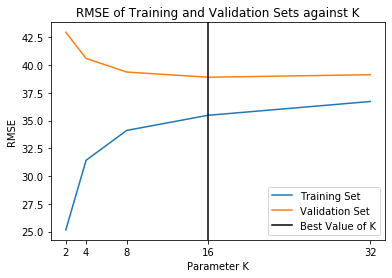
\includegraphics[width=1.0\textwidth]{figure8.png}
    \end{center}
}



\end{subquestion}

\begin{subquestion}{(1 points) What is the best-case RMSE performance on the validation set for KNN?}



\answerbox{6em}{
    The best case performance on the validation set is when $K=16$, with an $\mathrm{RMSE}$ value of 38.902.
}



\end{subquestion}

\begin{subquestion}{(4 points) Let us try one last regression algorithm: we will now use \href{https://scikit-learn.org/stable/modules/generated/sklearn.tree.DecisionTreeRegressor.html}{DecisionTreeRegressor}. Again, the algorithm contains a number of hyper-parameters, and we will optimise the depth of the tree. Train a series of Decision Tree Regressors, optimising (over the validation set) the \texttt{max\_depth} over the values [2, 4, 8, 16, 32, 64]. Set \texttt{random\_state=0}. Plot the training/validation RMSE and indicate (as before) the best value for \texttt{max\_depth}.}



\answerbox{40em}{
    \begin{center}
        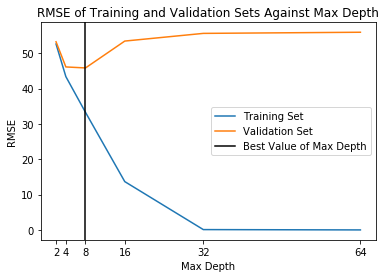
\includegraphics[width=1.0\textwidth]{figure9.png}
    \end{center}
}



\end{subquestion}

\begin{subquestion}{(3 points) What is the best-case RMSE performance on the validation set? What do you notice from the plot about the performance of the Decision Tree Regressor?}



\answerbox{6em}{
    The best case performance on the validation set is when $\mathrm{max\_depth}=8$, with an $\mathrm{RMSE}$ value of 45.844. As the max depth increases the decision tree model starts to overfit to the training data more and more. This causes poor predictions on unseen data, which can be seen from the $\mathrm{RMSE}$ value of the validation set increasing.
}



\end{subquestion}

\begin{subquestion}{(5 points) To conclude let us now compare all the models on the testing set. Combine the training and validation sets and retrain the model from each family on it: in cases where we optimised hyper-parameters, set this to the best-case value. Report the testing-set performance of each model in a table \hint{You should have 4 values}.}



\answerbox{6em}{
    \resizebox{0.77\textwidth}{!}{\begin{minipage}{\textwidth}
        \begin{tabular}{lrrrr}
            \toprule
            {} &  Baseline Regressor &  Linear Regression &  KNN Regression &  Decision Tree Regressor \\
            \midrule
            RMSE of Testing Set &           78.937312 &          40.509027 &       37.984965 &                43.068871 \\
            \bottomrule
        \end{tabular}
    \end{minipage}}
}



\end{subquestion}

\end{question}

%============================================================================


\end{document}
